\documentclass[dvipdfmx,a4paper,11pt]{jsbook}


% 数式
\usepackage{amsmath,amsfonts}
\usepackage{mathtools}
\usepackage{xcolor}
\usepackage{xcoffins,calc}
\usepackage{bm}
\usepackage{amsthm}
\usepackage{amssymb}
\usepackage{pgf}
\usepackage{tcolorbox}
\usepackage{titlesec}
\usepackage{ifthen}
\usepackage{mathrsfs}

% 画像
% \usepackage[dvipdfmx]{graphicx,color}

\usepackage[%
dvipdfmx, %欧文ではコメントアウトする
setpagesize=false,
bookmarks=true,
bookmarksdepth=tocdepth,
bookmarksnumbered=true,
colorlinks=true,
linkcolor=blue,
citecolor=blue,
urlcolor=blue,
pdftitle={},
pdfsubject={},
pdfauthor={},
pdfkeywords={}
]{hyperref}

\usepackage{pxjahyper}
\usepackage{tikz}
\usetikzlibrary{intersections,calc,arrows.meta}
\usepackage[truedimen,top=25truemm,bottom=30truemm,hmargin=25truemm]{geometry}
\usepackage{calc}
\usepackage{fancyhdr}
\pagestyle{fancy}


\pagestyle{fancy}
\fancyhf{} % 全てのヘッダーとフッターをクリア
\fancyhead[LE,RO]{\thepage} % 左側の偶数ページと右側の奇数ページにページ番号を表示
\fancyhead[RE]{\leftmark} % 右側の偶数ページに章名を表示
\fancyhead[LO]{\rightmark} % 左側の奇数ページに節名を表示
\renewcommand{\headrulewidth}{0.4pt} % ヘッダーの線の太さを設定
\renewcommand{\footrulewidth}{0pt} % フッターの線の太さを定

% \makeatletter
% \let\old@rule\@rule
% \def\@rule[#1]#2#3{\textcolor{blue}{\old@rule[#1]{#2}{#3}}}
% \makeatother
% \newtcolorbox{mybox}[2][]{enhanced,skin=enhancedlast jigsaw,
% attach boxed title to top left={xshift=-4mm,yshift=-0.5mm},
% fonttitle=\bfseries\sffamily,varwidth boxed title=0.7\linewidth,
% colbacktitle=blue!45!white,colframe=red!50!black,
% interior style={top color=blue!10!white,bottom color=red!10!white},
% boxed title style={empty,arc=0pt,outer arc=0pt,boxrule=0pt},
% underlay boxed title={
% \fill[blue!45!white] (title.north west) -- (title.north east)
% -- +(\tcboxedtitleheight-1mm,-\tcboxedtitleheight+1mm)
% -- ([xshift=4mm,yshift=0.5mm]frame.north east) -- +(0mm,-1mm)
% -- (title.south west) -- cycle;
% \fill[blue!45!white!50!black] ([yshift=-0.5mm]frame.north west)
% -- +(-0.4,0) -- +(0,-0.3) -- cycle;
% \fill[blue!45!white!50!black] ([yshift=-0.5mm]frame.north east)
% -- +(0,-0.3) -- +(0.4,0) -- cycle; },
% title={#2},#1}

% chapter 
\titleformat{\chapter}[block]
{}{}{0pt}{
  \ifthenelse{\value{chapter}=0}{}
  {\vspace*{-2cm}}\fontsize{27pt}{30pt}\selectfont\filleft
}[
  \ifthenelse{\value{chapter}=0}{\hrule}{\titleline{
  \hspace{225pt}
  \begin{tikzpicture}
    \draw [thick,line width = 0.4pt] (0,0) -- (7.5cm,0);
    \draw [thick,line width = 0.4pt] (6.5cm,2cm)-- (6.5cm,-1cm);
    % \draw [line width = 0.4pt] (6.5cm,1cm) -- (6.5cm,-1cm);
  \end{tikzpicture}}}
  \Large{\filleft \ifthenelse{\value{chapter}=0}{}{\vspace*{-1cm}第 \thechapter 章}}
]



\makeatletter
\def\Section{\@ifstar{\@Section[2pt]}{\@Section[\z@]}}
%
\def\@Section[#1]#2{\ifdim #1<1pt\refstepcounter{section}\fi%
\section*{\nopagebreak[4] \vskip.5pc%
\ifdim #1<1pt%
\addcontentsline{toc}{section}{\protect\numberline{\thesection}#2}%
\quad \textbf{\thesection~} \fi \raisebox{-1.5ex}[0pt][0pt]{\color[rgb]{0.6,0.8,1}{\rule{3mm}{2em}}} #2\nopagebreak[4]%
\vskip.25pc \hrule\@height 1pt\nopagebreak[4] \vskip1pc}}
\makeatother

% % 定理環境の設定
\tcbuselibrary{skins, breakable, theorems}
\usepackage{cleveref}
% \newcommand{\kara}{}
% \newtcolorbox[auto counter, number within = section, crefname = {Def.}{Defs.}]{definition}[3][]{enhanced, breakable = true, fonttitle = \bfseries,title = Def.~\thetcbcounter~\if #2\kara \else (#2) \fi, #1, label = the:#3, boxrule=0pt, frame hidden, borderline west={4pt}{0pt}{green!75!black},
% colback=green!10!white,sharp corners}



% \newtheorem{theorem}{Theorem}[section]
% \tcolorboxenvironment{theorem}{
%   colback=blue!5!white,
%   boxrule=0pt,
%   boxsep=1pt,
%   left=2pt,right=2pt,top=2pt,bottom=2pt,
%   oversize=2pt,
%   sharp corners,
%   before skip=\topsep,
%   after skip=\topsep,
% }




\renewcommand{\qedsymbol}{$\blacksquare$}
\newcommand{\Claim}[1]{\underline{\textbf{Claim#1.}}}

\newcommand{\kara}{}%
\newcounter{totalcounter}
\renewcommand{\thetotalcounter}{\thechapter.\thesection.\arabic{totalcounter}}
\newcounter{defcounter}
\renewcommand{\thedefcounter}{\thechapter.\thesection.\arabic{defcounter}}

\NewTotalTColorBox[use counter = defcounter, number within = section]{\Definition}{ +m }{ 
    notitle,
    colback=green!5!white,
    frame hidden,
    boxrule=0pt,
    enhanced,
    sharp corners,
    borderline west={4pt}{0pt}{green!50!black},
    breakable = true,
    label = {Def:\thedefcounter},
}{
    \textcolor{green!50!black}{
        \sffamily
        \textbf{Definition~\thetcbcounter.}%k
    }%
    #1
}

\NewTotalTColorBox{\Remark}{ +m +m }{ 
    notitle,
    colback=yellow!5!white,
    colbacklower=white,
    frame hidden,
    boxrule=0pt,
    bicolor,
    sharp corners,
    borderline west={4pt}{0pt}{yellow!50!black},
    %fontupper=\sffamily,
    breakable = true,
    label = {Rem:\thetotalcounter},
}{
    \textcolor{yellow!50!black}{
        \sffamily
        \textbf{Remark~.}%
    }%
    #1
    \if #2\kara \else 
    \tcblower%
    \textcolor{yellow!50!black}{
        \sffamily
        \textbf{Proof.}%
    }%
    #2
    \qedsymbol
    \fi
}

\NewTotalTColorBox[use counter = totalcounter, number within = section]{\Lemma}{ +m +m }{ 
    notitle,
    colback=orange!5!white,
    colbacklower=white,
    frame hidden,
    boxrule=0pt,
    bicolor,
    sharp corners,
    borderline west={4pt}{0pt}{orange!50!black},
    fontupper=\sffamily,
    breakable = true,
    label = {Lem:\thetotalcounter},
}{
    \textcolor{orange!50!black}{
        \sffamily
        \textbf{Lemma~\thetcbcounter.}%
    }%
    #1
    \if #2\kara \else 
    \tcblower%
    \textcolor{orange!50!black}{
        \sffamily
        \textbf{Proof.}%
    }%
    #2
    \qedsymbol
    \fi
}


\NewTotalTColorBox[use counter = totalcounter, number within = section]{\Theorem}{ +m +m }{ 
    notitle,
    colback=blue!5!white,
    colbacklower=white,
    frame hidden,
    boxrule=0pt,
    bicolor,
    sharp corners,
    borderline west={4pt}{0pt}{blue!50!black},
    fontupper=\sffamily,
    breakable = true,
    label = {Thm:\thetotalcounter},
}{
    \textcolor{blue!50!black}{
        \sffamily
        \textbf{Theorem~\thetcbcounter.}%
    }%
    #1
    \if #2\kara \else 
    \tcblower%
    \textcolor{blue!50!black}{
        \sffamily
        \textbf{Proof.}%
    }%
    #2
    \qedsymbol
    \fi
}

\NewTotalTColorBox[use counter = totalcounter, number within = section]{\Example}{ +m +m }{ 
    notitle,
    colback=cyan!5!white,
    colbacklower=white,
    frame hidden,
    boxrule=0pt,
    bicolor,
    sharp corners,
    borderline west={4pt}{0pt}{cyan!50!black},
    %fontupper=\sffamily,
    breakable = true,
    label = {Ex:\thetotalcounter},
}{
    \textcolor{cyan!50!black}{
        \sffamily
        \textbf{Example~\thetcbcounter.}%
    }%
    #1
    \if #2\kara \else
    \tcblower%
    \textcolor{cyan!50!black}{
        \sffamily
        \textbf{Proof.}%
    }%
    #2
    \qedsymbol
    \fi
}

\NewTotalTColorBox[use counter = totalcounter, number within = section]{\Proposition}{ +m +m }{ 
    notitle,
    colback=red!5!white,
    colbacklower=white,
    frame hidden,
    boxrule=0pt,
    bicolor,
    sharp corners,
    borderline west={4pt}{0pt}{red!50!black},
    fontupper=\sffamily,
    breakable = true,
    label = {Prop:\thetotalcounter},
}{
    \textcolor{red!50!black}{
        \sffamily
        \textbf{Proposition~\thetcbcounter.}%
    }%
    #1
    \if #2\kara \else 
    \tcblower%
    \textcolor{red!50!black}{
        \sffamily
        \textbf{Proof.}%
    }%
    #2
    \qedsymbol
    \fi
}
\NewTotalTColorBox[use counter = totalcounter, number within = section]{\Corollary}{ +m +m }{ 
    notitle,
    colback=darkgray!5!white,
    colbacklower=white,
    frame hidden,
    boxrule=0pt,
    bicolor,
    sharp corners,
    borderline west={4pt}{0pt}{darkgray!50!black},
    fontupper=\sffamily,
    breakable = true,
    label = {Cor:\thetotalcounter},
}{
    \textcolor{darkgray!50!black}{
        \sffamily
        \textbf{Corollary~\thetcbcounter.}%
    }%
    #1
    \if #2\kara \else 
    \tcblower%
    \textcolor{darkgray!50!black}{
        \sffamily
        \textbf{Proof.}%
    }%
    #2
    \qedsymbol
    \fi
}

% \newtcbtheorem[use counter from = theorem]{mythm}{Theorem}%
% {
%   colback=white, % ボックス内の背景色
%   colframe=black, % フレームの色
%   fonttitle=\bfseries, % タイトルのフォント
% }{thm}

% % 証明環境の設定
% \newtcbtheorem[use counter from = theorem]{mypf}{Proof}%
% {
%   colback=white, 
%   colframe=black, 
%   fonttitle=\bfseries
% }{prf}

% % 定義環境の設定
% \newtcbtheorem[use counter from = theorem]{mydef}{Definition}%
% {
%   colback=white, 
%   colframe=black, 
%   fonttitle=\bfseries
% }{def}

\newtcolorbox{mybox}{
  enhanced,
  boxrule=0pt,frame hidden,
  borderline west={4pt}{0pt}{green!75!black},
  colback=green!10!white,
  sharp corners
}

\newcommand{\mysetminusD}{\hbox{\tikz{\draw[line width=0.6pt,line cap=round] (3pt,0) -- (0,6pt);}}}
\newcommand{\mysetminusT}{\mysetminusD}
\newcommand{\mysetminusS}{\hbox{\tikz{\draw[line width=0.45pt,line cap=round] (2pt,0) -- (0,4pt);}}}
\newcommand{\mysetminusSS}{\hbox{\tikz{\draw[line width=0.4pt,line cap=round] (1.5pt,0) -- (0,3pt);}}}

\newcommand{\mysetminus}{\mathbin{\mathchoice{\mysetminusD}{\mysetminusT}{\mysetminusS}{\mysetminusSS}}}

\newcommand{\defi}{\stackrel{\mathrm{def}}{\equiv}}
\renewcommand{\ker}[1]{\mathrm{Ker}\, #1}
\newcommand{\im}[1]{\mathrm{Im}\, #1}
\newcommand{\coker}[1]{\mathrm{Coker}\, #1}
\renewcommand{\hom}[3]{\mathrm{Hom}_{#1}(#2,#3)}


\begin{document}

% \setlength{\topmargin}{-20truemm}
% \setlength{\headheight}{0pt}
% \setlength{\headsep}{0pt}
\setlength{\footskip}{20truemm}



% \setlength{\@tempdima}{1pt*\ratio{\dimexpr\textheight/\@lines}{\baselineskip}}
% \renewcommand{\baselinestretch}{\strip@pt\@tempdima}\selectfont

\makeatletter
\newcount\@chars\newcount\@lines
\@chars=40                      % 1行の文字数
\@lines=40                      % 1ページの行数

\newdimen\@kanjiskip
\@kanjiskip=\dimexpr(\textwidth-1zw*\@chars)/\numexpr\@chars-1
\newdimen\@@kanjiskip
\@@kanjiskip=\dimexpr\@kanjiskip/10

\baselineskip=\dimexpr\textheight/\@lines
\kanjiskip=\@kanjiskip plus \@@kanjiskip minus \@@kanjiskip
\parindent=\dimexpr 1zw+2truept
\parindent=\dimexpr\parindent+\@kanjiskip
\makeatother

% ↑は貼り付けただけなのでわからない.



\title{代数幾何まとめノート}
\date{\today}
\author{Fefr}
\maketitle




\tableofcontents
\clearpage
%--------------------本文--------------------%

\chapter{Scheme}
\Section{Zariski Topology}
atodekakuyo
\Section{Algebraic Sets}
atodekakuyo
\Section{Sheaves}
\Definition{
  $X$を位相空間とする.$X$上の(アーベル群の)\textbf{前層}(presheaf)$\, \mathcal{F}$とは
  次のデータ
  \begin{center}
    \begin{itemize}
      \item[---] $U$を任意の$X$の開集合に対して$\mathcal{F}(U)$はアーベル群.
      \item[---] 制限写像(restriction map)と言われる群準同型
            $\rho_{U,V}:\mathcal{F}(U) \to \mathcal{F}(V)$が任意の開集合$V\subset U$に対して存在する.
    \end{itemize}
  \end{center}
  そして次の条件を満たす.
  \begin{itemize}
    \item[(1)] $\rho_{U,U} = \text{id}_{\mathcal{F}(U)}$
    \item[(2)] 任意の開集合$W\subset V \subset U$に対して$\rho_{U,W}=\rho_{V,W}\circ \rho_{U,V}$となる.
  \end{itemize}
}
$s\in \mathcal{F}(U)$を$U$上の$\mathcal{F}$の\textbf{切断}(section)という.
また,$\rho_{U,V}(s)\in \mathcal{F}(V)$を$s|_{V}$と書いて$s$の$V$への制限という.\\
また,単に$\mathcal{F,G,H,}\dots$などと書いたら(前)層を表すことや、$\rho$と書いたら制限写像を意味する。
また,どの(前)層の制限写像かを明示するため,例えば,$\rho_{U,V}^{\mathcal{F}}$などと書くことがある。
\Definition{
  前層$\mathcal{F}$が層(sheaf)とは次の条件を満たすことをいう.
  \begin{itemize}
    \item[(4)] (Uniqueness) $U$を$X$の開集合とし$\{U_{i}\}_{i}$をその開被覆とする.
          $s\in \mathcal{F}(U)$が任意の$i$に対して$s|_{U_{i}}=0$ならば$s=0$
    \item[(5)] (Glueing local sections) 上の状況で,$s_i \in \mathcal{F}(U_i)$が
          $s_{i}|_{U_{i} \cap U_{j}} = s_{j}|_{U_{i} \cap U_{j}}$を満たすならば,$s|_{U_{i}} = s_{i}$を満たす$s\in \mathcal{F}(U)$が存在する.
  \end{itemize}
}
\Remark{
  $\mathcal{F}$が層ならば$\mathcal{F}(\varnothing) = 0$となる.
}{}
\Example{
$X$を位相空間とする.\\
$\mathcal{C}_{X}^{0}$を$X$の開集合$U$に対して$U\to \mathbf{C}$なる連続写像全体の集合$\mathcal{C}_{X}^{0}(U)$を対応させるものとし,制限写像を普通の制限とする.
すると,$\mathcal{C}_{X}^{0}$は$X$上の層となる.
}{
$V \subset U$なる開集合$U,V$に対して$U$上の連続写像$f\in \mathcal{C}_{X}^{0}(U)$を$V$に制限することによって得られる
$V$上の連続写像を$\rho_{U,V}(f)(=f|_{V})$と書く.すると,これは$\mathbf{C}$上のベクトル空間($\mathbf{C}$上の関数空間)
の準同型$\rho_{U,V}:\mathcal{C}_{X}^{0}(U) \to \mathcal{C}_{X}^{0}(V)$となる.つまり$(\mathcal{C}_{X}^{0},\rho)$は前層となる.\\
また,(4)を満たすのは明らかで.(5)もすぐに成り立つことがわかる.$\{U_{i}\}_{i}$を$U$の開被覆とする.$f_{i} \in \mathcal{C}_{X}^{0}(U_{i})$が
$f_{i}|_{U_{i} \cap U_{j}} = f_{j}|_{U_{i} \cap U_{j}}$を満たすとする.するとそれらを張り合わせた関数を$f$とすればこれは
$f\in \mathcal{C}_{X}^{0}(U)$であり,$f|_{U_{i}}=f_{i}$となる.よって$(\mathcal{C}_{X}^{0},\rho)$は層となる.これを連続写像が成す層という.
}
\Example{
$X$を位相空間とする.\\
$A$を自明でないアーベル群とする.$\mathcal{A}_{X}$を$X$の空でない開集合$U$に対して$\mathcal{A}_{X}(U)=A$に,
空集合$\varnothing$に対して$\mathcal{A}_{X}(\varnothing) = 0$に対応させるものとし,
制限写像を空でない開集合$V \subset U$に対して$\rho_{U,V}=\text{id}_{A}$とし,$\rho_{U,\varnothing} = 0$とする.\\
すると,$(\mathcal{A}_{X},\rho)$は$X$上の前層にはなるが,一般に層とはならない.\\
}{
例えば,$X$が連結でないとすると,非交差な開集合$U,V$があって$X=U\cup V$とかける.すると$\{U,V\}$は$X$の開被覆となる.
$s_{U} \in \mathcal{A}_{X}(U)=A$が$s_{U}|_{U\cap V} = s_{U}|_{\varnothing} = 0 = s_{V}|_{U \cap V}$
を満たすとする.このとき,任意の$s \in \mathcal{A}_{X}(X)=A$で$s|_{U}=s|_{V}=s$となり層とならない.
}

\Example{
  (skyscraper sheaf)\\
  $X$を位相空間、$A$をアーベル群とする。$p\in X$に対して$i_{p} : \{p\} \hookrightarrow X$を包含写像とする。
  このとき$i_{p,*}\mathcal{A}$を
  \begin{equation*}
    i_{p,*}\mathcal{A}(U) = \left\{ 
    \begin{alignedat}{2}
      &A \qquad &p \in U\\
      &1 \qquad &p \notin U
    \end{alignedat}
    \right.
  \end{equation*}
  と定義する。これは層になる。
}{}

\Remark{
$\mathcal{B}$を位相空間$X$の開基で有限交叉で閉じているものとする.(つまり任意の$U,V\in \mathcal{B}$に対して$U\cap V \in \mathcal{B}$.\ e.g. $\text{Spec}\, A$の開基$\{D(f)\}_f$)
このとき$\mathcal{B}$-前層($\mathcal{B}\text{-presheaf}$)\\$\mathcal{F}'$とは
  \begin{itemize}
    \item[---] $U\in \mathcal{B}$に対して$\mathcal{F}'(U)$はアーベル群.
    \item[---] $V\subset U \in \mathcal{B}$に対して群準同型$\rho_{U,V}:\mathcal{F}'(U) \to \mathcal{F}'(V)$が定まる.
  \end{itemize}
  としたもの.\\
$\mathcal{B}$-層($\mathcal{B}\text{-sheaf}$)$\mathcal{F}'$から$X$上の層$\mathcal{F}$を作ることができる.\\
% 位相空間$X$の任意の開集合$U$をとり,$\{U_{i}\}_{i}$をその開被覆とする.($U_{i} \in \mathcal{B}$)
% \begin{equation*}
%   \mathcal{F}(U):=\left\{(s_{i})_{i} \in \prod_{i}\mathcal{F}_0(U_{i})\ \Biggl|\ 任意のi,jに対してs_{i}|_{U_{i} \cap U_{j}} = s_{j}|_{U_{i} \cap U_{j}}\right\}
% \end{equation*}
% と定義する.するとこれは開被覆によらない.実際$\mathcal{F}(U)_{U_i}$を開被覆$\{U_{i}\}_{i}$による$\mathcal{F}(U)$とし,$\{V_{j}\}_{j}$を別の開被覆とすると,
% $\{U_{i}\cap V_{j}\}_{i,j}$はこれら2つの細分である.$\mathcal{F}(U)_{U_i} \to \mathcal{F}(U)_{U_{i}\cap V_{j}}$なる群準同型を
% $(s_{i})_{i}\mapsto (s_{i}|_{U_{i}\cap V_{j}})_{i,j}$で定義できる.実際
% \begin{align*}
%   s_{i} |_{U_{i} \cap V_{j}}\Bigl|_{(U_{i} \cap V_{j}) \cap (U_{i'} \cap V_{j'})}
%     & = s_{i} \Bigl|_{(U_{i} \cap V_{j}) \cap (U_{i'} \cap V_{j'})}                                                                              \\
%     & = s_{i} |_{U_{i}\cap U_{i'}}\Bigl|_{(U_{i} \cap V_{j}) \cap (U_{i'} \cap V_{j'})}                                                          \\
%     & = s_{i'} |_{U_{i}\cap U_{i'}}\Bigl|_{(U_{i} \cap V_{j}) \cap (U_{i'} \cap V_{j'})} \quad (\because (s_{i})_{i} \in \mathcal{F}(U)_{U_{i}}) \\
%     & = s_{i'} \Bigl|_{(U_{i} \cap V_{j}) \cap (U_{i'} \cap V_{j'})}                                                                             \\
%     & = s_{i'} |_{U_{i'} \cap V_{j'}}\Bigl|_{(U_{i} \cap V_{j}) \cap (U_{i'} \cap V_{j'})}
% \end{align*}
% より$(s_{i}|_{U_{i}\cap V_{j}})_{i,j}\in \mathcal{F}(U)_{U_{i} \cap V_{j}}$\\
% また,$(s_{ij})_{ij}\in \mathcal{F}(U)_{U_{i}\cap V_{j}}$を取ると,
% $(s_{ij})_{ij} = (s_{i}|_{U_{i} \cap V_{j}})$と出来るので全射(?????)\\
% Kernelを計算すると
% \begin{align*}
%     & s_{i}|_{U_{i}\cap V_{j}} = 0 \quad (\forall i,j)                \\
%     & s_{i}|_{U_{i}}=s_{i} = 0 \quad (\forall i) \quad (\because (4))
% \end{align*}
% よってKernelが自明なので単射.
% % $\mathcal{U}=\{U_{i}\}_{i}$を$X$の部分開集合族とする.$U=\cup_{i}U_{i},U_{ij}=U_{i}\cap U_{j}$


位相空間$X$の任意の開集合$V$に対して
\begin{align*}
  \mathcal{F}(V) 
  &= \varprojlim_{\substack{U\in \mathcal{B}\\ U\subset V}}\mathcal{F}'(U)\\
  &= \left\{(s_{U})_{U} \in \prod_{\substack{U\in \mathcal{B}\\ U \subset V}} \mathcal{F}'(U) \ \biggl|\ 
  \forall U' \subset U \in \mathcal{B}, s_{U}|_{U'}=s_{U'} \right\}
\end{align*}
と定める.制限写像は射影極限から誘導される射である.
\begin{center}
  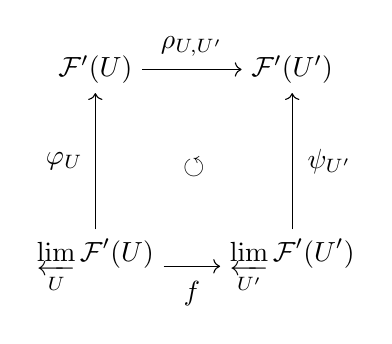
\begin{tikzpicture}[auto]
    \node (X1) at (0,0) {$\mathcal{F}'(U)$};
    \node (X2) at (0,-2.5) {$\displaystyle \varprojlim_{U}\mathcal{F}'(U)$};
    \node (Y1) at (2.5,0) {$\mathcal{F}'(U')$};
    \node (Y2) at (2.5,-2.5) {$\displaystyle \varprojlim_{U'}\mathcal{F}'(U')$};
    \node (ci) at (1.25,-1.25) {$\circlearrowleft$};

    \draw[->] (X1) to node[yshift = -6pt,label=above:$\rho_{U,U'}$] () {} (Y1);
    \draw[->] (X2) to node[xshift = 6pt, label=left:$\varphi_{U}$] () {} (X1);
    \draw[->] (X2) to node[yshift = -2pt,label=below:$f$] () {} (Y2);
    \draw[->] (Y2) to node[xshift = 2pt,label=right:$\psi_{U'}$] () {} (Y1);
  \end{tikzpicture}
\end{center}
% F(V)とF(V')にしてU'ではなくU\cap V'にしよう.
これが層となることを確かめよう.まず,任意の開集合$V$とその開被覆$\{U_{i}\}_{i}\subset \mathcal{B}$をとる.
$s\in \mathcal{F}(V)$に対して$s|_{U_{i}}=0$とする.すると定義から$U\subset V$なる任意の$U\in \mathcal{B}$に対して$s_{U}\in \mathcal{F}'(U)$が$0$であることを示せば$s=0$ということである.
実際$V$の開被覆から$U$の開被覆$\{U \cap U_{i}\}_{i}\subset \mathcal{B}$が得られる.
また任意の$i$に対して$U\cap U_{i} \subset U_{i}$より$s_{U_{i}}|_{U\cap U_{i}} = s_{U\cap U_{i}} = 0$となる.(いま$s_{U_{i}}$は$s|_{U_{i}}$のこと)
したがって任意の$i$に対して$s_{U}|_{U\cap U_{i}} = 0$となる.いま$\mathcal{F}'$は層なので$s_{U}=0$
よって$s=0$がわかった.\\
また,$s_{i} \in \mathcal{F}(U_{i})$が$s_{i}|_{U_{i}\cap U_{j}} = s_{j}|_{U_{i} \cap U_{j}}$を満たすとする.
よって,$U_{i}\cap U_{j} \in \mathcal{B}$より
}{}


\Definition{
  位相空間$X$上の前層$\mathcal{F}$と$x\in X$に対して,$x$での$\mathcal{F}$の\textbf{茎(stalk)}$\mathcal{F}_{x}$という群が定義できる.
  \begin{equation*}
    \mathcal{F}_{x} = \varinjlim_{U \ni x}\mathcal{F}(U)
  \end{equation*}
  ただし,$U$は$x$の開近傍をすべてを回る.$U$上の切断$s\in \mathcal{F}(U)$に対して
  $x\in U$の茎$\mathcal{F}_{x}$への自然な群準同型の像を$s_{x}$と書いて,$x$での$s$の\textbf{芽(germ)}という.
}
\Lemma{
$\mathcal{F}$を$X$上の層とする.$s,t \in \mathcal{F}(X)$が任意の$x \in X$に対して$s_{x} = t_{x}$ならば$s=t$
}{
差を考えれば$t=0$のときを考えればいい.$s_{x}=0\ (\forall x\in X)$とすると,$x$の開近傍$U_{x}$があって$s|_{U_{x}}=0$となる.$\{U_{x}\}_{x\in U_{x}}$は$X$の開被覆なので,$s=0$となる.
}
\Definition{
$X$上の2つの前層$\mathcal{F,G}$とする.\textbf{前層の射}$\alpha:\mathcal{F} \to \mathcal{G}$
とは,$X$の開集合$U$に対して群準同型$\alpha(U):\mathcal{F}(U) \to \mathcal{G}(U)$があって,
任意の開集合の組$V\subset U$に対して$\alpha(V)\circ \rho_{U,V}^{\mathcal{F}} = \rho_{U,V}^{\mathcal{G}}\circ \alpha(U)$を満たすことをいう.\\
$X$の任意の開集合$U$に対して$\alpha(U)$が単射ならば$\alpha$は単射であるという.(全射はうまくいかんっぽい?)
}

$\alpha:\mathcal{F} \to \mathcal{G}$を$X$上の前層の射とする.任意の$x \in X$に対して
$\alpha$から自然に誘導される群準同型$\alpha_{x}:\mathcal{F}_{x} \to \mathcal{G}_{x}$で
$(\alpha(U)(s))_{x} = \alpha_{x}(s_{x})$が$X$の任意の開集合$U,s\in \mathcal{F}(U),x\in U$で
成り立つものが取れる.\\
$\alpha_{x}$が任意の$x\in X$で全射なら$\alpha$が全射であるという.

\Example{
  $X=\mathbf{C} \mysetminus \{0\}$とし$\mathcal{F}$を$X$上の正則関数がなす層とし,
  $\mathcal{G}$を$X$上の双正則関数のなす層とする.今,任意の開集合$U$と任意の$f\in \mathcal{F}(U)$に対して$\alpha(U)(f) = \exp(f)$で定義される層の射$\alpha:\mathcal{F} \to \mathcal{G}$
  が全射であることはよく知られている.しかし$\alpha(X):\mathcal{F}(X) \to \mathcal{G}(X)$は
  全射ではない.例えば恒等写像は$\exp(f)$と書けない.
}{}
\Proposition{
  $\alpha:\mathcal{F} \to \mathcal{G}$を$X$上の層の射とする.
  \begin{center}
    $\alpha$が同型$\Leftrightarrow$ $\alpha_{x}$が同型$(\forall x \in X)$
  \end{center}
}{}
\Theorem{
位相空間$X$上の前層$\mathcal{F}$に対して,前層$\mathcal{F}$の層化(sheafification)$\mathcal{F}^{\dagger}$は存在する.
}{
$X$の開集合$U$に対して
\begin{equation*}
  \mathcal{F}^{\dagger}(U) = \left\{\sigma: U \to \prod_{x\in U} \mathcal{F}_{x}\, \middle|\,
  \begin{aligned}
    \forall x\in U,x\in \exists V\subset U:\text{open},\exists s \in \mathcal{F}(V)\, \text{s.t.}\, \sigma(y) = s_{y}\, (\forall y \in V)
  \end{aligned}
  \right\}
\end{equation*}
とする.ただし,$\sigma$は任意の$x\in U$に対して$\sigma(x) \in \mathcal{F}_{x}$とする.
また,$V \subset U$なる開集合に対し,
$$
  \begin{array}{rccc}
    \rho_{U,V}^{\mathcal{F}^{\dagger}}: & \mathcal{F}^{\dagger}(U) & \longrightarrow & \mathcal{F}^{\dagger}(V) \\
                                        & \rotatebox{90}{$\in$}    &                 & \rotatebox{90}{$\in$}    \\
                                        & \sigma                   & \longmapsto     & \sigma|_{V}
  \end{array}
$$
が定義できる.実際,任意の$x\in V$をとる.$V \subset U$であり,
$\sigma \in \mathcal{F}^{\dagger}(U)$より
\begin{center}
  $x\in \exists U_{0} \subset U$:open,$\exists s \in \mathcal{F}(U_{0})$\, s.t.\, $\sigma(y)=s_{y}\, (\forall y\in U_{0})$
\end{center}
$V_{0} = U_{0} \cap V,\quad t = s|_{V_{0}}$とすると任意の$y\in V_{0}$に対して
\begin{equation*}
  \sigma(y)=\sigma|_{V}(y)=s_{y}
\end{equation*}
さらに帰納極限の定義から
\begin{equation*}
  \sigma|_{V}(y)=t_{y}
\end{equation*}
次に$\mathcal{F}^{\dagger}(U)$がアーベル群,つまり
$\sigma,\tau \in \mathcal{F}^{\dagger}(U)$ならば$\sigma+\tau \in \mathcal{F}^{\dagger}(U)$
を示そう.\\
$\sigma,\tau \in \mathcal{F}^{\dagger}(U)$より任意の$x\in U$に対して
\begin{align*}
    & x\in \exists U_{0} \subset U:\mathrm{open},\exists s \in \mathcal{F}(U_{0})\ \mathrm{s.t.}\
  \sigma(y) = s_{y}\ (\forall y \in U_{0})                                                       \\
    & x\in \exists V_{0} \subset U:\mathrm{open},\exists t \in \mathcal{F}(V_{0})\ \mathrm{s.t.}\
  \tau(z) = t_{z}\ (\forall z \in V_{0})
\end{align*}
を満たす.いま$W = U_{0} \cap V_{0},s' = s|_{W},t' = t|_{W}$とすると,
\begin{align*}
  x\in W \subset U:\mathrm{open}, s',t' \in \mathcal{F}(W)\ \mathrm{s.t.}\
  (\sigma + \tau)(y)
    & = \sigma(y) + \tau(y)             \\
    & = s_{y} + t_{y}                   \\
    & = (s + t)_{y} \ (\forall y \in W)
\end{align*}
よって$\sigma + \tau \in \mathcal{F}^{\dagger}(U)$また明らかに可換.
よって$\mathcal{F}^{\dagger}(U)$はアーベル群.\\
また,通常の制限で制限写像を定義しているため,$\mathcal{F}^{\dagger}$は前層となる.\\
更に層となることを示そう.\\
$U$を$X$の開集合とし,$\{U_{i}\}_{i}$をその開被覆とする.$\sigma\in \mathcal{F}^{\dagger}(U)$が
任意の$i$に対して$\sigma|_{U_{i}} = 0$とする.つまり任意の$x \in U_{i}$に対して$\sigma(x) = 0$
とする.$U_{i}$は$U$を被覆するので結局$\sigma = 0$となる.\\
次に,$\sigma_{i} \in \mathcal{F}^{\dagger}(U_{i})$とし,
$\sigma_{i}|_{U_{i} \cap U_{j}} = \sigma_{j}|_{U_{i} \cap U_{j}}$と仮定すると,
$$
  \begin{array}{rccc}
    \sigma : & U                     & \longrightarrow & \displaystyle \prod_{x\in U}\mathcal{F}_{x} \\
              & \rotatebox{90}{$\in$} &                 & \rotatebox{90}{$\in$}                       \\
              & x                     & \longmapsto     & \sigma_{i}(x)
  \end{array}
$$
ただし,$x\in U_{i}$.すると,$\sigma$は$\sigma_{i}\in \mathcal{F}^{\dagger}(U_{i})$を張り合わせて作っているので
これは$\sigma \in \mathcal{F}(U)$となることが容易にわかる。よって、$\mathcal{F}^{\dagger}$は層になる。
}



\Proposition{
  層化の射$\theta:\mathcal{F} \to \mathcal{F}^{\dagger}$に対して、
  その茎の射$\theta_{x}:\mathcal{F}_{x} \to \mathcal{F}^{\dagger}_{x}$は同型である。
}{}



\Lemma{
  $\mathcal{F}$を$X$上の層とし、$\mathcal{F}'$を$\mathcal{F}$の部分層とする。
  このとき開集合$U$を$\mathcal{F}(U)/\mathcal{F}'(U)$に対応させるものは前層になる。
}{
  この対応を$\mathcal{G}$とおく。$V \subset U$なる開集合$U,V$をとる。制限写像を
  $$
    \begin{array}{rccc}
      \rho_{U,V}^{\mathcal{G}} : & \mathcal{F}(U)/\mathcal{F}'(U) & \longrightarrow & \mathcal{F}(V)/\mathcal{F}'(V)                \\
                                  & \rotatebox{90}{$\in$}          &                 & \rotatebox{90}{$\in$}                         \\
                                  & s + \mathcal{F}'(U)            & \longmapsto     & \rho_{U,V}^{\mathcal{F}}(s) + \mathcal{F}'(V)
    \end{array}
  $$
  とすると、これはwell-definedである。また、$U\subset V \subset W$なる開集合の組に対して
  \begin{equation*}
    \rho_{U,W}^{\mathcal{G}} = \rho_{V,W}^{\mathcal{G}} \circ \rho_{U,V}^{\mathcal{G}}
  \end{equation*}
  が成り立つことは制限写像の定義から明らかである。よって$\mathcal{G}$は前層。
}
\Definition{
  Lem:\ref{Lem:1.3.8}で定義した前層の層化を$\mathcal{F}/\mathcal{F}'$と書いて、\textbf{商層(quotient shaef)}という。
}
\Definition{
  $\alpha:\mathcal{F} \to \mathcal{G}$を前層の射とする。このとき開集合$U$に対して
  $U \mapsto \ker (\alpha(U))$とするものは$\mathcal{F}$の部分層になる。これを$\ker{\alpha}$と
  書いて、\textbf{$\alpha$の核(kernel of $\alpha$)}という。\\
  更に、$U\mapsto \im (\alpha(U))$は一般には前層となるので、これの層化を$\im \alpha$と書いて、
  \textbf{$\alpha$の像(image of $\alpha$)}という。\\
  また,$U\mapsto \coker (\alpha(U)) = \mathcal{G}(U)/\im (\alpha(U))$は一般には前層となるので,これの層化を$\coker \alpha$と書いて,\textbf{$\alpha$の余核(cokernel of $\alpha$)}という.
}
\Lemma{
  $\mathcal{F,G}$を$X$上の層,$\mathcal{F}'$を$\mathcal{F}$の部分層,$\alpha:\mathcal{F} \to \mathcal{G}$を前層の射とする。
  このとき、
  \begin{align*}
      & (\ker \alpha)_{x} = \ker \alpha_{x}                               \\
      & (\im \alpha)_{x} = \im \alpha_{x}                                 \\
      & (\coker \alpha)_{x} = \coker \alpha_{x} \\
      & (\mathcal{F}/\mathcal{F}')_{x} = \mathcal{F}_{x}/\mathcal{F}'_{x}
  \end{align*}
  が成り立つ。
}{
  $\mathcal{Q}(U) = \mathcal{F}(U)/\mathcal{F}'(U)$とおく。\\
  このとき、アーベル群の完全列
  \begin{center}
    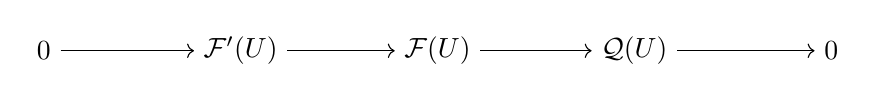
\begin{tikzpicture}[auto]
      \node (03) at (0,-1) {$0$};
      \node (im1) at (2.5,-1) {$\mathcal{F}'(U)$};
      \node (gu) at (5,-1) {$\mathcal{F}(U)$};
      \node (qu) at (7.5,-1) {$\mathcal{Q}(U)$};
      \node (04) at (10,-1) {$0$};

      \draw[->] (03) to (im1);
      \draw[->] (im1) to (gu);
      \draw[->] (gu) to (qu);
      \draw[->] (qu) to (04);
    \end{tikzpicture}
  \end{center}
  が作れる。帰納極限は完全列を完全列に移すので、またProp:\ref{Prop:1.3.7}より
  \begin{center}
    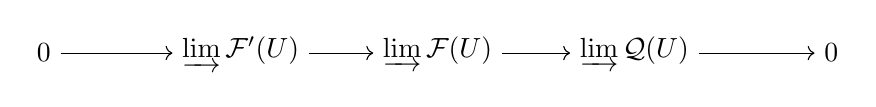
\begin{tikzpicture}[auto]
      \node (03) at (0,-1) {$0$};
      \node (im1) at (2.5,-1) {$\varinjlim \mathcal{F}'(U)$};
      \node (gu) at (5,-1) {$\varinjlim \mathcal{F}(U)$};
      \node (qu) at (7.5,-1) {$\varinjlim \mathcal{Q}(U)$};
      \node (04) at (10,-1) {$0$};

      \draw[->] (03) to (im1);
      \draw[->] (im1) to (gu);
      \draw[->] (gu) to (qu);
      \draw[->] (qu) to (04);
    \end{tikzpicture}
  \end{center}
  を得る。よって
  \begin{center}
    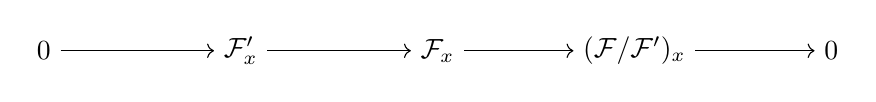
\begin{tikzpicture}[auto]
      \node (03) at (0,-1) {$0$};
      \node (im1) at (2.5,-1) {$\mathcal{F}'_{x}$};
      \node (gu) at (5,-1) {$\mathcal{F}_{x}$};
      \node (qu) at (7.5,-1) {$(\mathcal{F}/\mathcal{F}')_{x}$};
      \node (04) at (10,-1) {$0$};

      \draw[->] (03) to (im1);
      \draw[->] (im1) to (gu);
      \draw[->] (gu) to (qu);
      \draw[->] (qu) to (04);
    \end{tikzpicture}
  \end{center}
  したがって、
  \begin{equation*}
    \mathcal{F}_{x}/\mathcal{F}'_{x} \simeq (\mathcal{F}/\mathcal{F}')_{x}
  \end{equation*}
  を得る。\\
  次に
  \begin{align*}
    (\ker \alpha)_{x}
      & = \{s_{x} \in \mathcal{F}_{x} \ |\ \alpha(U)(s) = 0,x\in U:\text{open},s\in \mathcal{F}(U) \}   \\
      & = \{s_{x} \in \mathcal{F}_{x} \ |\ \alpha_{x}(s_{x})=0,x\in U:\text{open},s\in \mathcal{F}(U)\} \\
      & = \ker \alpha_{x}
  \end{align*}
  を得る。同様に
  \begin{align*}
    (\im \alpha)_{x}
      & = \{t_{x} \in \mathcal{G}_{x} \ |\ x\in \exists U:\text{open}, \exists s\in \mathcal{F}(U)\ \text{s.t}\ t = \alpha(U)(s)\} \\
      & = \{(\alpha(U)(s))_{x} \in \mathcal{G}_{x} \ |\ x \in U:\text{open},s\in \mathcal{F}(U)\}                                  \\
      & = \{\alpha_{x}(s_{x}) \in \mathcal{G}_{x}\ |\ s_{x} \in \mathcal{F}_{x}\}                                                  \\
      & = \im \alpha_{x}
  \end{align*}
  を得る.また,$(\mathcal{F}/\mathcal{F}')_{x} = \mathcal{F}_{x}/\mathcal{F}'_{x}$より
  \begin{equation*}
    (\coker \alpha)_{x} = (\mathcal{G}/\im \alpha)_{x} = \mathcal{G}_{x}/\im \alpha_{x} = \coker \alpha_{x}
  \end{equation*}
}

\Definition{
  層の列
  \begin{equation*}
    \mathcal{F} \stackrel{\alpha}{\longrightarrow} \mathcal{G} \stackrel{\beta}{\longrightarrow} \mathcal{H}
  \end{equation*}
  が完全とは、$\im \alpha = \ker \beta$が成り立つことをいう。
}
\Proposition{
  層の列に対して次が成り立つ。
  \begin{equation*}
    \mathcal{F} \longrightarrow \mathcal{G} \longrightarrow \mathcal{H}が完全
    \Longleftrightarrow
    任意のx \in Xに対して\mathcal{F}_{x} \longrightarrow \mathcal{G}_{x} \longrightarrow \mathcal{H}_{x}が完全
  \end{equation*}
}{
  明らか。
}

\Definition{
  $X,Y$を位相空間,$f:X\to Y$を連続写像とする。このとき、
  $X$上の層$\mathcal{F}$,$Y$上の層$\mathcal{G}$に対して、新たな$Y$上の層$f_{*}\mathcal{F}$が
  \begin{equation*}
    V \mapsto \mathcal{F}(f^{-1}(V))
  \end{equation*}
  によって定義できる。これを\textbf{$\mathcal{F}$の順像(direct image of $\mathcal{F}$)}という。\\
  また、
  \begin{equation*}
    U \mapsto \varinjlim_{V\supset f(U)}\mathcal{G}(V)
  \end{equation*}
  で定義できる新たな$X$上の前層$f^{\cdot}\mathcal{G}$の層化$f^{*}\mathcal{G}$を\textbf{$\mathcal{G}$の逆像(inverse image of $\mathcal{G}$)}
  という。
}

\Proposition{
  上の状況で
  \begin{equation*}
    (f^{*}\mathcal{G})_{x} = \mathcal{G}_{f(x)} \qquad \forall x \in X
  \end{equation*}
}{
  \begin{equation*}
    (f^{*}\mathcal{G})_{x} = \varinjlim_{x \in U}(f^{*}\mathcal{G})(U) = \varinjlim_{x \in U}\varinjlim_{f(U) \subset V}\mathcal{G}(V) = \mathcal{G}_{f(x)}
  \end{equation*}
  最後の等号は明らか.
}

\Remark{
  $V$を$Y$の開集合とする。このとき自然な単射$i:V \to Y$に対して
  \begin{equation*}
    i^{*}\mathcal{G} = \mathcal{G}|_{V}
  \end{equation*}
  が成り立つ。
}{}
\Proposition{
  $f:X \to Y$を位相空間の間の連続写像とし,$\mathcal{F}$を$X$上の層.$\mathcal{G}$を$Y$上の層とする.このとき
  \begin{equation*}
    \hom{\text{Sh}(X)}{f^{*}\mathcal{G}}{\mathcal{F}}\simeq \hom{\text{Sh}(Y)}{\mathcal{G}}{f_{*}\mathcal{F}}
  \end{equation*}
  ただし,$\hom{\mathcal{C}}{X}{Y}$は圏$\mathcal{C}$で$X \to Y$なる射全体を表し,$\text{Sh}(X)$は$X$上の層全体を表す.
}{
  層化の普遍性より$\theta:f^{\cdot}\mathcal{G} \to f^{*}\mathcal{G} = (f^{\cdot}\mathcal{G})^{\dagger}$
  を層化の射とすると,
  $$
  \begin{array}{rccc}
     & \hom{\text{PreSh}(X)}{f^{\cdot}\mathcal{G}}{\mathcal{F}}                     & \stackrel{\simeq}{\longrightarrow} & \displaystyle \hom{\text{Ph(X)}}{f^{*}\mathcal{G}}{\mathcal{F}} \\
              & \rotatebox{90}{$\in$} &                 & \rotatebox{90}{$\in$}                       \\
              & \alpha                     & \longmapsto     & \tilde{\alpha}\circ \theta
  \end{array}
  $$
  が成り立つ.つまり
  \begin{equation*}
    \hom{\text{PreSh}(X)}{f^{\cdot}\mathcal{G}}{\mathcal{F}}\simeq \hom{\text{Sh(Y)}}{\mathcal{G}}{f_{*}\mathcal{F}}
  \end{equation*}
  を示せばいい.次に$X$上の開集合$U$に対して
  \begin{equation*}
    f^{\cdot}\mathcal{G}(U) = \varinjlim_{V\supset f(U)}\mathcal{G}(V)
  \end{equation*}
  なので,$\varphi \in \hom{\text{PreSh}(X)}{f^{\cdot}\mathcal{G}}{\mathcal{F}}$に対して
  \begin{equation*}
    \varphi(U) : \varinjlim_{V\supset f(U)}\mathcal{G}(V) \to \mathcal{F}(U)
  \end{equation*}
  を与えることは帰納極限の定義より$f(U)\subset V$なる開集合$V$に対して
  \begin{equation*}
    \psi'(V) : \mathcal{G}(V) \to \mathcal{F}(U)
  \end{equation*}
  を$f(U)\subset V' \subset V$ならば,
  \begin{equation*}
    \psi'(V) = \psi'(V')\circ \rho^{\mathcal{G}}_{V,V'}
  \end{equation*}
  となるように与えることである.すなわち$\psi'(V)$は
  \begin{equation*}
    \psi(V):\mathcal{G}(V) \to \mathcal{F}(f^{-1}(V))
  \end{equation*}
  と$\rho^{\mathcal{F}}_{f^{-1}(V),U}$を合成したものである.(帰納系の選び方によらない.)\\
  したがって,$\varphi\in \hom{\text{PreSh}(X)}{f^{\cdot}\mathcal{G}}{\mathcal{F}}$を与えることは,$\psi \in \hom{\text{Ph}(Y)}{\mathcal{G}}{f_{*}\mathcal{F}}$を与えることと等しい.
}








\Section{Ringed Topological Space}

\Definition{
  \textbf{局所環付き空間}とは位相空間$X$と$X$上の環の層$\mathcal{O}_{X}$の組$(X,\mathcal{O}_{X})$
  で、任意の$x\in X$に対して$\mathcal{O}_{X,x}$が局所環となるものをいう。また、この$\mathcal{O}_{X}$
  を$(X,\mathcal{O}_{X})$の\textbf{構造層(structure sheaf)}という。また$(X,\mathcal{O}_{X})$を単に
  $\mathcal{O}_{X}$と書くことがある。\\
  また、$\mathcal{O}_{X,x}$の唯一の極大イデアル$\mathfrak{m}_{x}$に対して
  その剰余体$\mathcal{O}_{X,x}/\mathfrak{m}_{x}$を\textbf{$X$の点$x$での剰余体(residue field of X at x)}といって$k(x)$と書く。
}

\Definition{
  局所環付き空間の射とは
  \begin{equation*}
    (f,f^{\#}): (X,\mathcal{O}_{X}) \to (Y,\mathcal{O}_{Y})
  \end{equation*}
  とは連続写像$f:X \to Y$と環の層の射$f^{\#}:\mathcal{O}_{Y} \to f_{*}\mathcal{O}_{X}$の組$(f,f^{\#})$で、
  任意の$x\in X$に対して$f^{\#}_{x} : \mathcal{O}_{Y,f(x)} \to \mathcal{O}_{X,x}$は局所射となるものをいう。(つまり$f^{\#}_{x}(\mathfrak{m}_{Y,f(x)})\subset \mathfrak{m}_{X,x}$を満たす.)
}
Prop:\ref{Prop:1.3.13}より
\begin{equation*}
  f^{\#} : \mathcal{O}_{Y} \to f_{*}\mathcal{O}_{X}
\end{equation*}
を考えることは
\begin{equation*}
  f^{\#} : f_{*}\mathcal{O}_Y \to \mathcal{O}_{X}
\end{equation*}
を考えることに等しい.Def:\ref{Def:1.4.2}の$f^{\#}_{x}$は下の式で考えている.

\Definition{
  射$(f,f^{\#}):(X,\mathcal{O}_{X}) \to (Y,\mathcal{O}_{Y})$が\textbf{開はめ込み(open immersion)}(resp. \textbf{閉はめ込み(closed immersion)})
  とは連続写像$f$が開はめ込み(resp. 閉はめ込み)
  \footnote{$f:X\to Y$が(位相的)開(閉)はめ込みとは$X$と$f(X)$が同相で$f(X)$が開(閉)集合のときをいう。}
  でかつ任意の$x\in X$に対して$f^{\#}_{x}$が同型(resp. 全射)のときをいう。
}

\Definition{
  $(X,\mathcal{O}_{X})$を局所環付き空間とする。$\mathcal{J}$が$\mathcal{O}_{X}$の
  \textbf{イデアル層(sheaf of ideals of $\mathcal{O}_{X}$)}とは任意の開集合$U$に対して
  $\mathcal{J}(U)$が$\mathcal{O}_{X}(U)$のイデアルになっているときをいう。
}

\Lemma{
  $(X,\mathcal{O}_{X})$を局所環付き空間とする。$\mathcal{J}$を$\mathcal{O}_{X}$のイデアル層とする。
  そして、
  \begin{equation*}
    V(\mathcal{J}) = \{x \in X\ |\ \mathcal{J}_{x} \neq \mathcal{O}_{X,x}\}
  \end{equation*}
  とおく。(ちなみに上の諸々から$\mathcal{J}_{x} \subset \mathcal{O}_{X,x}$が分かる。)\\
  $j:V(\mathcal{J}) \hookrightarrow X$を包含写像とする。すると
  \begin{itemize}
    \item[---] $V(\mathcal{J})$は$X$の閉集合
    \item[---] $(V(\mathcal{J}),j^{*}(\mathcal{O}_{X}/\mathcal{J}))$は局所環付き空間
    \item[---] $j^{\#}$は自然な全射
    \begin{equation*}
      \mathcal{O}_{X} \longrightarrow \mathcal{O}_{X}/\mathcal{J} = j_{*}(j^{*}(\mathcal{O}_{X}/\mathcal{J}))
    \end{equation*}
    で
    $(j,j^{\#}):(V(\mathcal{J}),j^{-1}(\mathcal{O}_{X}/\mathcal{J})) \to (X,\mathcal{O}_{X})$は閉はめ込みである。
  \end{itemize}
}{
  \Claim{1}$V(\mathcal{J})$は$X$の閉集合\\
  $x\in X\mysetminus V(\mathcal{J}) = \{x\in X\ |\ \mathcal{J}_{x} = \mathcal{O}_{X,x}\}$
  に対して$f_{x} = 1$なる$x$の開近傍$U$と$f\in \mathcal{J}(U)$をとる。
  つまり$f|_{V} = 1|_{V} = 1$なる$x$の開近傍$V \subset U$がある。
  すると任意の$y \in V$に対して$f_{y} = 1 \in \mathcal{J}_{y}$となって,この$y$に対して
  $\mathcal{J}_{y} = \mathcal{O}_{X,y}$なので
  $V\subset X \mysetminus V(\mathcal{J})$となって$X\mysetminus V(\mathcal{J})$が開であることがわかる。\\
  \Claim{2}$(V(\mathcal{J}),j^{*}(\mathcal{O}_{X}/\mathcal{J}))$は局所環付き空間\\
  任意の$x\in V(\mathcal{J})$に対して
  \begin{equation*}
    (j^{*}(\mathcal{O}_{X}/\mathcal{J}))_{x} = (\mathcal{O}_{X}/\mathcal{J})_{x} = \mathcal{O}_{X,x}/\mathcal{J}_{x}
  \end{equation*}
  は局所環。残りは自明。
}

\Proposition{
  $f:X \to Y$を局所環付き空間の閉はめ込みとする。$Z$を局所環付き空間$V(\mathcal{J})$とする。
  ただし、$\mathcal{J} = \ker f^{\#}\subset \mathcal{O}_{Y}$.すると$X\simeq Z$を自然な閉はめ込み
  $Z \hookrightarrow Y$から得る。
}{
まず次の完全列
  \begin{equation*}
    0 \longrightarrow \mathcal{J} \longrightarrow \mathcal{O}_{Y} \longrightarrow f_{*}\mathcal{O}_{X} \longrightarrow 0
  \end{equation*}
  からProp:\ref{Prop:1.3.11}より任意の$y \in Y$に対して
  \begin{equation*}
    \mathcal{O}_{Y,y}/\mathcal{J}_{y} = (f_{*}\mathcal{O}_{X})_{y}
  \end{equation*}
  を得る。よって
  \begin{equation*}
    (f_{*}\mathcal{O}_{X})_{y} = \left\{ 
    \begin{alignedat}{2}
      &\quad 0 \qquad &y& \in Y \mysetminus V(\mathcal{J})\\
      &\mathcal{O}_{Y,y}/\mathcal{J}_{y} \qquad &y& \in V(\mathcal{J})
    \end{alignedat}
    \right.\qquad \cdots (*)
  \end{equation*}
  を得る。$f(X)$は$Y$の閉集合なので$x\in Y\mysetminus f(X)$の開近傍$U$で
  \begin{equation*}
    f(X)\cap U = \varnothing
  \end{equation*}
  となるものがとれる。よって
  \begin{equation*}
    f_{*}\mathcal{O}_{X}(U) = \mathcal{O}_{X}(f^{-1}(U)) = \mathcal{O}_{X}(\varnothing) = 0
  \end{equation*}
  したがって、
  \begin{equation*}
    (f_{*}\mathcal{O}_{X})_{x} = 0
  \end{equation*}
  また、$x\in f(X)$の開近傍$U$に対して$f$での引き戻し$f^{-1}(U)$は$y=f(x)$の開近傍である。
  これを$V$とおく。逆に、$f$は閉はめ込みなので、$X$は$f(X)$と同相なので$X$に自然に$Y$の相対位相が入る。
  つまり、任意の$x\in X$の開近傍$U$に対して$y=f(x)\in Y$の開近傍$V$が存在して$f^{-1}(V)$とかける。
  よって、
  \begin{equation*}
    (f_{*}\mathcal{O}_{X})_{x} = \varinjlim_{U \ni x}f_{*}\mathcal{O}_{X}(U) = \varinjlim_{U \ni x}\mathcal{O}_{X}(f^{-1}(U)) = \varinjlim_{V \ni y}\mathcal{O}_{X}(V) = \mathcal{O}_{X,y}
  \end{equation*}
  つまり、
  \begin{equation*}
    (f_{*}\mathcal{O}_{X})_{y} = \left\{ 
    \begin{alignedat}{2}
      &\quad 0 \qquad &y& \in Y \mysetminus f(X)\\
      &\mathcal{O}_{X,x} \qquad &y& = f(x)
    \end{alignedat}
    \right.
  \end{equation*}
  $(*)$と比較すれば
  \begin{equation*}
    V(\mathcal{J}) = f(X)
  \end{equation*}
  が分かる。
  なので、$j:Z \hookrightarrow Y$を包含写像とすると、$f$から誘導される同相写像$g:X \to Z$に対して
  \begin{equation*}
    f = j \circ g
  \end{equation*}
  で、
  \begin{equation*}
    j_{*}\mathcal{O}_{Z} = \mathcal{O}_{Y}/\mathcal{J} \simeq f_{*}\mathcal{O}_{X}
  \end{equation*}
  がわかる。容易に
  \begin{equation*}
    f_{*}\mathcal{O}_{X} = j_{*}g_{*}\mathcal{O}_{X}
  \end{equation*}
  が分かるので
  \begin{equation*}
    \mathcal{O}_{Z} = (j^{-1}\circ j)_{*}\mathcal{O}_{Z} = (j^{-1})_{*}j_{*}\mathcal{O}_{Z}\simeq (j^{-1})_{*}j_{*}g_{*}\mathcal{O}_{X} = (j^{-1}\circ j)_{*} g_{*}\mathcal{O}_{X} = g_{*}\mathcal{O}_{X}
  \end{equation*}
  である。よって、$g$は局所環付き空間の同型射である。$f=j\circ g$が局所環付き空間の射であることを確認するのは読者に委ねる。
}



\Section{Schemes}

\Proposition{
  $A$を環、$X=\text{Spec}\, A$とする。このとき以下が成り立つ。
  \begin{itemize}
    \item[(1)] $\mathcal{O}_{X}'$を環の$\mathfrak{B}$-層とする。$\mathcal{O}_{X}'$が誘導する$X$上の層$\mathcal{O}_{X}$は$\mathcal{O}_{X}(X)=A$となる。
    \item[(2)] 任意の$\mathfrak{p}\in X$に対して、茎$\mathcal{O}_{X,\mathfrak{p}}$は$A_{\mathfrak{p}}$への標準的な同型がある。特に、$(X,\mathcal{O}_{X})$は局所環付き空間になる。 
  \end{itemize}
}{
  まず,開集合$U=X$についてUniquness条件を確認する.ほかの基本開集合も同様に示される.
  $U_{i} = $
}

\Definition{
  上で定義した局所環付き空間$(\text{Spec}\, A,\mathcal{O}_{\text{Spec}\, A})$を
  \textbf{アフィンスキーム(affine scheme)}という.
}

\Lemma{
  $A$を整域とし$K$をその商体とする.素イデアル$0$に対応する$X = \text{Spec}\, A$の点を$\xi$とする.このとき
  \begin{equation*}
    \mathcal{O}_{X,\xi} = K
  \end{equation*}
  が成り立つ.さらに,任意の空でない開集合$U \subset X$と$\xi \in U$に対して
}{}





  \clearpage
  \appendix
  \chapter{Limit}
  \Section{Inductive Limit}
  とりあえず,帰納極限だけ述べる.射影極限は双対概念なのでまぁ頑張って.
  \Definition{(帰納系の定義)\\
  ($\Lambda,\leq$)を順序集合,$\mathscr{C}$を圏とする.各$\lambda \in \Lambda$に対し,$X_{\lambda} \in \text{Ob}(\mathscr{C})$が与えられ,
$\lambda \leq \mu$に対して射$\varphi_{\mu,\lambda}:X_{\lambda} \to X_{\mu}$があって
  次を満たすとき,$\{X_{\lambda},\varphi_{\mu,\lambda}\}$を\textbf{順系(direct system)}または
  \textbf{帰納系(inductive system)}という.しばし$\varphi_{\mu,\lambda}$を省略して$\{X_{\lambda}\}_{\lambda \in \Lambda}$や$\{X_{\lambda}\}_{\lambda}$で表す.
  \begin{itemize}
    \item[---] 任意の$\lambda \in \Lambda$に対して$\varphi_{\lambda,\lambda}=\text{id}_{X_{\lambda}}$
    \item[---] $\lambda \leq \mu \leq \nu$なる任意の$\lambda,\mu,\nu \in \Lambda$に対して$\varphi_{\nu,\lambda} = \varphi_{\nu,\mu}\circ \varphi_{\mu,\lambda}$
  \end{itemize}
  }
  \Example{
  位相空間$X$の開集合族$\{U\}_{U}$に対して
  \begin{equation*}
    U \leq V \defi V \subset U
  \end{equation*}
  と定義する.そして,$\mathbf{AGrp}$をアーベル群の成す圏,$\mathcal{F}$を$X$上の前層とする.すると,各開集合$U$に対し,$\mathcal{F}(U) \in \mathrm{Ob}(\mathbf{AGrp})$で,
  前層の定義からアーベル群と制限写像との組$\{\mathcal{F}(U),\rho_{U,V}\}$は帰納系となる.前層の定義はDef:\ref{Def:1.3.1}を参照.
  }{}
  \Definition{(帰納系の射の定義)\\
$\Lambda$を順序集合.$\{X_{\lambda},\varphi_{\lambda,\mu}\},\{Y_{\lambda},\psi_{\lambda,\mu}\}$を$\Lambda$上の圏$\mathscr{C}$における帰納系とする.
  このとき$\{X_{\lambda}\}$から$\{Y_{\lambda}\}$への射とは$f_{\lambda}:X_{\lambda} \to Y_{\lambda}$なる射の族
$\{f_{\lambda}\}$で,任意の$\lambda \leq \mu$に対して
$\psi_{\lambda,\mu}\circ f_{\mu} = f_{\lambda}\circ \varphi_{\lambda,\mu}$となるものを言う.
  %---------------後に図式を追加する.------------------%
  \begin{center}
    \begin{tikzpicture}[auto]
      \node (X1) at (0,0) {$X_{\mu}$};
      \node (X2) at (0,-2.5) {$X_{\lambda}$};
      \node (Y1) at (2.5,0) {$Y_{\mu}$};
      \node (Y2) at (2.5,-2.5) {$Y_{\lambda}$};
      \node (ci) at (1.25,-1.25) {$\circlearrowleft$};

      \draw[->] (X1) to node[yshift = -6pt,label=above:$f_{\mu}$] () {} (Y1);
      \draw[->] (X1) to node[label=left:$\varphi_{\lambda,\mu}$] () {} (X2);
      \draw[->] (X2) to node[yshift = -2pt,label=below:$f_{\lambda}$] () {} (Y2);
      \draw[->] (Y1) to node[xshift = -6pt,label=right:$\psi_{\lambda,\mu}$] () {} (Y2);
    \end{tikzpicture}
  \end{center}
  }
  \Definition{
$\mathscr{C}$を圏とし,$\Lambda$を順序集合とする.$\{X_{\lambda},\varphi_{\mu,\lambda}\}$を
$\mathscr{C}$の帰納系とする.\\
  このとき$\{X_{\lambda},\varphi_{\mu,\lambda}\}$の\textbf{順極限(direct limit)}または\textbf{帰納的極限(inductive limit)}または\textbf{帰納極限}とは,
$\mathscr{C}$の対象$\displaystyle \varinjlim_{\lambda \in \Lambda}X_{\lambda} \in \text{Ob}(\mathscr{C})$
  と射の族$\displaystyle \{\varphi_{\lambda}:X_{\lambda} \to \varinjlim_{\lambda \in \Lambda}X_{\lambda}\}_{\lambda \in \Lambda}$の組
$\{\varinjlim X_{\lambda},\varphi_{\lambda}\}$で,次の条件を満たすものをいう.
\begin{itemize}
  \item[---] $\lambda \leq \mu$に対して$\varphi_{\mu}\circ \varphi_{\mu,\lambda} = \varphi_{\lambda}$
  \item[---] $\lambda \leq \mu$に対して$f_{\mu}\circ \varphi_{\mu,\lambda} = f_{\lambda}$を満たす任意の射の族$\{f_{\lambda}:X_{\lambda} \to Y\}_{\lambda \in \Lambda}$に対して,
        $\displaystyle f:\varinjlim_{\lambda \in \Lambda}X_{\lambda} \to Y$が一意に存在して
        \begin{equation*}
          f\circ \varphi_{\lambda} = f_{\lambda}\quad (\forall \lambda \in \Lambda)
        \end{equation*}
        を満たす.
\end{itemize}
}
\Remark{
  一般の圏では帰納極限や射影極限は存在するとは限らない.しかし,存在するとすれば,同型を除いて一意である.
}{}
\Proposition{
  帰納極限は存在すれば,同型を除いて一意である.
}{
  証明は後で書く.
}



\clearpage
\chapter{Category Theory}


\end{document}